\documentclass[a4paper,11pt]{article}

\usepackage[T1]{fontenc}
\usepackage[utf8]{inputenc}
\usepackage{amsmath,amssymb,amsthm,textcomp}

\usepackage[
pdftitle={Topological Exercises}, 
pdfauthor={Lucas Moschen, Fundação Getulio Vargas},
colorlinks=true,linkcolor=blue,urlcolor=blue,citecolor=blue,bookmarks=true,
bookmarksopenlevel=2]{hyperref}
\usepackage{enumerate}
\usepackage{multicol}
\usepackage{setspace}
\onehalfspacing

\usepackage{graphicx}
\usepackage{xcolor}
\usepackage{tikz}
\usepackage{float}
\usepackage{geometry}
\geometry{left=25mm,right=25mm,%
bindingoffset=0mm, top=20mm,bottom=20mm}

\newcommand{\linia}{\rule{\linewidth}{0.5pt}}

% custom theorems if needed
\newtheoremstyle{mytheor}
    {1ex}{1ex}{\itshape}{0pt}{\scshape}{.}{1ex}
    {{\thmname{#1 }}{\thmnumber{#2}}{\thmnote{ (#3)}}}

\theoremstyle{mytheor}
\newtheorem{definition}{Definition}[subsection]

\theoremstyle{mytheor}
\newtheorem{exercise}{Exercise}

\theoremstyle{remark}
\newtheorem*{remark}{Remark}

\newcommand{\T}{\mathcal{T}}
\newcommand{\U}{\mathcal{U}}
\newcommand{\B}{\mathcal{B}}
\newcommand{\Z}{\mathbb{Z}}
\newcommand{\R}{\mathbb{R}}
\newcommand{\sphere}{\mathbb{S}}

% my own titles
\makeatletter
\renewcommand{\maketitle}{
    \begin{center}
        \vspace{2ex}
        {\huge \textsc{\@title}}
        \vspace{1ex}
        \\
        \linia\\
        \@author \hfill \@date
        \vspace{4ex}
    \end{center}
}
\makeatother

%%%----------%%%----------%%%----------%%%----------%%%

\title{Topological Data Analysis - Exercises}

\author{Lucas Moschen, EMAp/FGV}

\date{\today}

\begin{document}

\maketitle

\tableofcontents

\section{General topology}

\subsection{Important definitions}

\begin{definition}
    A topological space is a pair $(X, \T)$ where $X$ is a set and $\T$ is a
    collection of subsets of $X$ such that:
    \begin{enumerate}
        \item $\emptyset \in \T, X \in \T$. 
        \item for every infinite collection $\{O_{\alpha}\}_{\alpha \in A}\subset \T$, we have $\bigcup_{\alpha \in A} O_{\alpha} \in \T$.
        \item for every finite collection $\{O_{i}\}_{1 \le i \le n}
        \subset \T$, we have $\bigcap_{1 \le i \le n} O_{i} \in \T$.
    \end{enumerate}   
\end{definition}

\begin{definition}
    Let $x \in \R^n$ and $r > 0$. The open ball of center $x$ and radius $r$,
    denoted $\B(x, r)$, is defined as: $\B(x, r) = \{y \in \R^n, ||x - y|| < r\}$.
\end{definition}

\begin{definition}
    Let $A \subset \R$ and $x \in A$. We say that $A$ is open
    around $x$ if there exists $r > 0$ such that $\B(x, r) \subset A$. We say
    that $A$ is open if for every $x \in A$, $A$ is open around $x$.
\end{definition}

\begin{definition}
    Let $(X, \T)$ be a topological space, and $Y \subset X$. We define the subspace topology on $Y$ as the following set:
    $$T_{|Y} = \{O \cap Y, O \in \T\}$$
\end{definition}

\begin{definition}
    Let $f : X \to Y$ be a map. We say that $f$ is continuous if for every
    $O \in U$, the preimage $f^{-1}(O) = \{x \in X, f(x) \in O\}$ is in $\T$.
\end{definition}

\subsection{Exercises}

\begin{exercise}
    Let $X = \{0, 1, 2\}$ be a set with three elements. What are the  different topologies that X admits?
\end{exercise}

As we know every Topology contains $\emptyset$ and $\{0,1,2\}$, so we can
disconsider when writing the topologies, that is, all below contain these
subsets. 

\begin{itemize}
    \item (2) Basic: $\{\emptyset, \{0,1,2\}\}$ - $\mathcal{P}(\{0,1,2\})$.  
    \item (8) With $\{0\}$: $\{\{0\}\} - \{\{0\}, \{0,1\}\} - \{\{0\}, \{1,2\}\} -
    \{\{0\}, \{0,2\}\} - \{\{0\}, \{0,2\}, \{0,1\}\}$ \\ 
    $\{\{0\}, \{2\}, \{0,2\}\}- \{\{0\}, \{2\}, \{0,2\}, \{1,2\}\} -
    \{\{0\}, \{2\}, \{0,2\}, \{0,1\}\}$

    \item (8) With $\{1\}$: $\{\{1\}\} - \{\{1\}, \{0,1\}\} - \{\{1\}, \{1,2\}\} -
    \{\{1\}, \{0,2\}\} - \{\{1\}, \{1,2\}, \{0,1\}\}$ \\
    $\{\{0\}, \{1\}, \{0,1\}\} - \{\{0\}, \{1\}, \{0,1\}, \{1,2\}\} -  \{\{0\}, \{1\}, \{0,1\}, \{0,2\}\}$

    \item (8) With $\{2\}$: $\{\{2\}\} - \{\{2\}, \{0,1\}\} - \{\{2\}, \{1,2\}\} -
    \{\{2\}, \{0,2\}\} - \{\{2\}, \{0,2\}, \{1,2\}\}$ \\
    $\{\{1\}, \{2\}, \{1,2\}\} - \{\{1\}, \{2\}, \{1,2\}, \{0,1\}\} - \{\{1\},
    \{2\}, \{1,2\}, \{0,2\}\}$ 
    
    \item (3) No singleton: $\{\{0,1\}\} - \{\{1,2\}\} - \{\{0,2\}\} $
\end{itemize}

\noindent\linia

\begin{exercise}
    Let $\Z$ be the set of integers. Consider the \textit{cofinite
    topology} $\T$ on $\Z$, defined as follows: a subset $O \subset
    \Z$ is an open set if and only if $O = \emptyset$ or $^c O$ is finite. Here, $^cO = \{x \in \Z, x \not\in O\}$ represents the complementary of $O$ in $\Z$
\end{exercise}

\begin{enumerate}
    \item Show that $\T$ is a topology on $\Z$.

    Let's verify the three axioms: 

    \begin{enumerate}
        \item $\emptyset$ is an open set by definition and $\Z$ is open set
        because $^c\Z = \emptyset$ is finite. 

        \item Let $\{O_{\alpha}\}_{\alpha \in A}\subset \T$. So 
        $^cO = ~^c\left(\bigcup_{\alpha \in A} O_{\alpha}\right) = \bigcap_{\alpha
        \in A} ~^cO_{\alpha} \implies ^c O \subset ~^cO_{\alpha}, \forall
        \alpha \in A$. If $\forall \alpha, O_{\alpha} = \emptyset$, then $^cO =
        ~^c\emptyset \implies O = \emptyset$   and $O$ is open. On the other
        hand, if there exists $\alpha \in A$ such that $O_{\alpha} \neq
        \emptyset$ we have $^c O_{\alpha}$ being finite, so is $^c O$, given
        the inclusion. We conclude $O$ is open set. 
        
        \item Let $\{O_{i}\}_{1 \le i \le n} \subset \T$. So 
        $^cO = ~^c\left(\bigcap_{1 \le i \le n} O_i\right) = \bigcup_{1 \le i
        \le n} ~^cO_i$. If $O_i = \emptyset$ for some $1 \le i \le n$, $O =
        \emptyset$ because of the intersection. Alternatively, if $\forall i,
        O_i \neq \emptyset$ we have that $^cO_i$ is finite and a finite union
        of finites is finite. We conclude that $O$ is open set.
    \end{enumerate}
    By (a), (b) and (c), $\T$ is a topology on $\Z$. 

    \item Exhibit an sequence of open sets $\{O_n\}_{n\in\mathbb{N}} \subset
    \T$ such that $\bigcap_{n \in \mathbb{N}} O_n$ is not an open
    set.

    Let $O_n = ~^c\{1, ..., n\}$. Thus $^c O_n = \{1,...,n\}$ is finite and
    $$^c\left(\bigcap_{n \in \mathbb{N}} O_n\right) = \bigcup_{n \in
    \mathbb{N}} ~^cO_n = \bigcup_{n \in
    \mathbb{N}} \{1,...,n\} = \mathbb{N},$$
    that is not finite. Therefore, this intersection is not an open set.     
    
\end{enumerate}

\noindent\linia

\begin{exercise}
    Let $x \in \R^n$, and $r > 0$. Let $y \in \B(x, r)$. Show that
    $$\B(y,r - ||x-y||) \subset \B(x,r)$$
\end{exercise}

Let $z \in \B(y, r - ||x-y||)$, so $||z - y|| < r - ||x - y|| \implies ||z-y||
+ ||x-y|| < r$. We can conclude
that, by the triangular inequality,  
$$||x - z|| \le ||x - y|| + ||z - y|| < r.$$ 
In that sense, $z \in \B(x,r)$ and $\B(y, r - ||x - y||) \subset \B(x,r)$.

\begin{remark}
    In the notes, the exercise is to prove $\B(y,||x-y||) \subset \B(x,r)$,
    however, this does not hold, because if we take $y$ next the border of
    $\B(x,r), ||x - y|| \approx r$ and $B(y,r -\epsilon) \not \subset B(x,r)$.
\end{remark}

\noindent\linia

\begin{exercise}
    Let $x, y \in \R^n$, and $r = ||x - y||$. Show that
    $$
    \B\left(\frac{x + y}{2}, \frac{r}{2}\right) \subset \B(x, r) \cap \B(y, r)
    $$
\end{exercise}

Denote $m = \dfrac{x+y}{2}$. Take $z \in \B\left(m, \dfrac{r}{2}\right)$.
Thus, using the triangular inequality,

$$||x - z|| \le ||x - m|| + ||m - z|| = \frac{1}{2}||x - y|| + ||m - z|| < r/2
+ r/2 = r$$
$$||y - z|| \le ||y - m|| + ||m - z|| = \frac{1}{2}||y - x|| + ||m - z|| < r/2
+ r/2 = r$$

So $z \in \B(x,r)$, $z \in \B(y, r)$ and $z \in \B(x,r) \cap \B(y, r)$.
Therefore $\B(m, \frac{r}{2}) \subset \B(x, r) \cap \B(y, r)$.

\noindent\linia

\begin{exercise}
    Show that the open balls $\B(x, r)$ of $R^n$ are open sets (with respect
    to the Euclidean topology).
\end{exercise}

We have to prove that for every $y \in \B(x, r)$, there exists $\epsilon > 0$ such
that $\B(y, \epsilon) \subset \B(x, r)$. Put $\epsilon = r - ||x - y||$. As
we have proved in exercise 3, $\B(y, \epsilon) \subset \B(x,r)$. 
So $\B(x,r)$ is open set. 

\noindent\linia

\begin{exercise}
    Consider $X = \R$ endowed with the Euclidean topology. Are the following
sets open? Are they closed?
\end{exercise}
\begin{enumerate}
    \item $[0,1]$. It's not open set because for every $\epsilon > 0, \B(0,
    \epsilon) = (-\epsilon, \epsilon) \not \subset [0,1]$. It's closed because
    $[0,1]^c = (-\infty, 0) \cup (1, \infty)$ is an union of two open sets, as
   we prove in item 3.  

    \item $[0,1)$. It's not open for the same reason as before. It's not
    closed because $B(1,\epsilon) = (1 - \epsilon, 1 + \epsilon) \not\subset
    (-\infty, 0) \cup [1, \infty]$. 

    \item $(-\infty,1)$. It's open because: take $x < 1$. Put $r = 1 - x$ and
    take $z \in \B(x, r)$. If $z > x$, $|x - z| < 1 - x \implies z < 1$. If $z
    < x$, it follows $z < 1$. It proves $z < 1$ and $(-\infty, 1)$ is open.
    It's not closed cause $\forall \epsilon > 0, \B(1,\epsilon) \not \subset
    [1, \infty)$. 
    
    \item the singletons. It's not open cause $\forall \epsilon > 0, x +
    \epsilon/2 \in \B(x,\epsilon)$. It's close cause $(-\infty,
    x)\cup(x,\infty)$ is union of open sets. 
    
    \item $\mathbb{Q}$. It's not open because for every open ball around a
    rational, there are irrationals, that is, let $x \in \mathbb{Q}$ and take
    $\epsilon > 0$, then there exists $y \in (\R - \mathbb{Q}) \cap
    \B(x,\epsilon)$. It's not closed for the same reason, for every
    irrational, there is rationals for every open ball. 

    \begin{remark}
        We shall prove the rationals are dense in the reals. Let $x \in
        \mathbb{Q}$ and $\epsilon > 0$. If $\epsilon$ is irrational, take $x-
        \epsilon/2 \subset (x - \epsilon, x + \epsilon)$. Suppose $x -
        \epsilon/2$ is rational, then $\frac{2x - \epsilon}{2} = \frac{m}{n}$
        for some integers $m$ and $n$, that is, $2x - \epsilon = 2m/n$ and
        $\epsilon = 2(x - \frac{m}{n}) \in \mathbb{Q}$, contradiction. So there
        is an irrational in $\B(x, \epsilon)$. If $\epsilon$ is rational,
        consider 
        $$y = \frac{1}{\sqrt{2}}(x - \epsilon) + (1 -
        \frac{1}{\sqrt{2}})(x + \epsilon) = (x + \epsilon) - \epsilon\sqrt{2}$$ 
        That is a convex combination, so
        $y \in \B(x, \epsilon)$. Moreover, $y$ is irrational, with a similar
        proof by contradiction. This proves the statement. 

        On the other hand, we must prove for every two irrationals $(a,b)$,
        there is a rational between them. Denote $c = b - a > 0$. Let $n\in
        \mathbb{N}$ such that $n > \frac{1}{c} \implies cn > 1 \implies (bn -
        an) > 1$. So exists $m \in (an, bn) \implies m/n \in (a,b)$. This
        proves the second statement.   
    \end{remark}
\end{enumerate}

\noindent\linia

\begin{exercise}
    A map is continuous if and only if the preimage of closed sets are closed sets.
\end{exercise}

First we shall prove that $f^{-1}(~^cA) = ~^c(f^{-1}(A))$. Let's prove the
double inclusion. Take $x \in f^{-1}(~^cA)$. So there exists $y \in ~^cA$ such
that $f(x) = y$. Suppose that $x \in f^{-1}(A)$. It implies the existence of
$z \in A$ such that $y = f(x) = z$, absurd. So $x \in ~^c(f^{-1}(A))$.

Now take $x \in ~^c(f^{-1}(A))$. Therefore, $\forall y \in A, f(x) \neq y$. In
that case, $f(x) \in ~^cA \implies x \in f^{-1}(~^cA)$. Then we have showed
the equality. 

\vspace{5mm}

Now let's prove the equivalence. Suppose $f$ is a continuos map and take a
closed set $F$. We shall prove that $f^{-1}(F)$ is closed. Well, $^c(f^{-1}(F))
= f^{-1}(~^cF)$ is open, because $~^cF$ is open, by the continuity. We
conclude that $f^{-1}(F)$ is closed. 

Suppose that for every closed set $F$, we have $f^{-1}(F)$ being closed. We
will use that $A$ is open if $^cA$ is closed. This is true because $^c(^c(A))
= A$. Take an open set $A$. $^c(f^{-1}(A)) = f^{-1}(~^cA)$
is closed, because $~^cA$ is. Thus $f^{-1}(A)$ is open and we have proved the
continuity of $f$. 


\newpage

\section{Homeomorphisms}

\subsection{Important definitions}

\begin{definition}
    Let $(X, \T)$ and $(Y, \U)$ be two topological spaces, and $f : X
    \to Y$ a map. We say that $f$ is a homeomorphism if
    \begin{enumerate}
        \item $f$ is a bijection, 
        \item $f : X \to Y$ is continuos, 
        \item $f^{-1} : Y \to X$ is continuos.
    \end{enumerate}
    If there exists such a homeomorphism, we say that the two topological
    spaces are homeomorphic.
\end{definition}

\begin{definition}
    Let $(X, \T)$ be a topological space. We say that $X$ is connected if for
    every open sets $O, O' \in \T$ such that $O \cap O' = \emptyset$ (i.e.,
    they are disjoint), we have
    $$X = O \cup O' \implies O = \emptyset \text{ or } O' = \emptyset.$$
\end{definition}

\begin{definition}
    Let $(X, \T)$ be a topological space. Suppose that there exists a
    collection of $n$ \textbf{non-empty}, \textbf{disjoint} and
    \textbf{connected open sets} $(O_1, ..., O_n)$ such that
    $$
    \bigcup_{1 \le i \le n} O_i = X.
    $$
    Then we say that $X$ admits $n$ connected components.
\end{definition}

\begin{definition}
    Let ($X, \T)$ be a topological space, and $n \geq 0$. We say that it has
    dimension $n$ if the following is true: for every $x \in X$, there exists
    an open set $O$ such that $x \in O$, and a homeomorphism $O \to \R^n$.
\end{definition}

\subsection{Exercises}

\begin{exercise}
    Show that the topological spaces $\R^n$ and $\B(0, 1) \subset \R^n$ are homeomorphic.
\end{exercise}

\begin{proof}

Let $f: \B(0,1) \to \R^n$ be defined as $f(x) = \dfrac{x}{1 - ||x||}$. I
observe it's well defined because $||x|| < 1$. We shall prove $f$ is a
homeomorphism. 
\begin{enumerate}
    \item \textbf{Injective:} Take $x, y \in \B(0,1)$ and suppose that  
    $$
    \frac{x}{1 - ||x||} = \frac{y}{1 - ||y||}. 
    $$
    Applying the norm in both sides, we obtain the equation 
    $$||x||(1 - ||y|||) = ||y||(1 - ||x||) \implies ||x|| = ||y||.$$
    On the other side $x$ and $y$ points to the same direction, given that 
    $$
    y = \frac{1 - ||y||}{1 - ||x||}x = \alpha x, 
    $$
    with $\alpha = 1$ because of the same norm. We conclude $x = y$. 

    \item \textbf{Surjective:} Take $y \in \R^n$. We shall prove that there
    exists $x \in \B(0,1)$ such that $f(x) = y$, that is, 
    $$
    \frac{x}{1 - ||x||} = y
    $$
    Applying the norm we observe that if that is true, $||x|| = ||y|| -
    ||y||||x|| \implies ||x|| = \frac{||y||}{1 + ||y||}$. And $x = (1 -
    ||x||)y = \frac{1}{1 + ||y||}y$. We conclude that for every $y \in \R^n$,
    if we take $x = \frac{y}{1 + ||y||}$,
    $$
    f(x) = \frac{y/(1 + ||y||)}{1 - ||y||/(1 + ||y||)} = y
    $$

    \item \textbf{Continuity of f:} Consider an open set $A \subset \R^n$. Let
    $B = f^{-1}(A)$. We shall prove $B$ is open, that is, for every $x \in B$,
    exists $r > 0$ such that $\B(x, r) \subset B$. Take $x = f^{-1}(y) \in B$.
    Because $A$ is open, there is $\epsilon > 0$ such that $\B(y, \epsilon)
    \subset A$. Take $\delta$ such that 
    $$
    \frac{\delta}{1 - ||x|| - \delta}(1 + ||y||) < \epsilon
    $$
    and $z = f^{-1}(w) \in \B(x,\delta)$. 
    \begin{equation*}
        \begin{split}
            ||y - w|| &= \left|\left|\frac{x}{1 - ||x||} - \frac{z}{1 - ||z||}\right|\right| = \frac{1}{1 - ||x||}\left|\left|x - \frac{1 - ||x||}{1 - ||z||}z\right|\right| \\ 
            &= \frac{1}{1 - ||x||}\left|\left|x - z + z - \frac{1 - ||x||}{1 - ||z||}z\right|\right| \\
            &\le \frac{||x-z||}{1 - ||x||} + \frac{1}{1 - ||x||}\left(1 - \frac{1 - ||x||}{1 - ||z||}||z||\right) \\
            &= \frac{||x-z||}{1 - ||x||} + \frac{||z||}{1 - ||x||}\frac{||x|| - ||z||}{1 - ||z||} \\
            &\le \frac{1}{1 - ||x||}||x-z||(1 + ||w||) \\
            &\le \frac{1}{1 - ||x||}||x-z||(1 + ||y - w|| + ||y||) \\
            \implies ||y - w|| &\le \frac{||x-z||}{1 - ||x|| - ||x-z||}(1 + ||y||) \\ 
            &< \frac{\delta}{1 - ||x|| - \delta}(1 + ||y||) < \epsilon
        \end{split}
    \end{equation*}
    So $w \in \B(y, \epsilon) \subset A \implies z \in B$, what proves $B$ is
    open. It concludes the continuity of $f$. 

    \item \textbf{Continuity of $f^{-1}$: } The inverse is given by 
    $$
    f^{-1}(y) = \frac{y}{1 + ||y||}
    $$
    The demonstration is quite similar to the previous item, given that the
    only difference is the signal. 
\end{enumerate}

By items (1) - (4), we conclude $f$ is a homeomorphism and $\B(0,1) \simeq
\R^n$.

\end{proof}

\noindent\linia

\begin{exercise}
    Show that $\B(x, r)$ and $\B(y, s)$ are homeomorphic.
\end{exercise}

\begin{proof}

Consider the function $f: \B(0, 1) \to \B(c, r)$ given by $f(x) = r\cdot x + c$. Let's
prove $f$ is a homeomorphism. 
\begin{enumerate}
    \item \textbf{Injective:} If $x,y \in \B(0,1)$ and $rx + c = ry + c
    \implies x = y$, because $r > 0$ by 
    definition. So $f$ is injective. 
    
    \item \textbf{Surjective:}  Let $y \in \B(c, r)$ and $x = (y - c)/r$. So
    $||x|| = ||y - c||/r < 1$, by definition. So $x \in \B(0,1)$ and $f(x) =
    y$ what proves this function is surjective. 

    \item \textbf{Continuity of f:} Let $A \subset \B(c,r)$ open set and
    denote $B = f^{-1}(A)$. Take $x = f^{-1}(y) \in B$. We know there exists
    $\epsilon > 0$ such that $\B(y, \epsilon) \subset A$. Define $\delta = \epsilon/r$ and
    take $z = f^{-1}(w) \in \B(x,\delta)$. 
    $$
    ||y-w|| = ||rx + c - (rz + c)|| = r||x - z|| < r\delta = \epsilon 
    $$
    Therefore $w \in \B(y, \epsilon) \subset A \implies z \in B$. So
    $\B(x,\delta) \subset B$, what proves $B$ is open. This concludes the
    continuity of $f$. 
    
    \item \textbf{Continuity of $f^{-1}$:} The inverse is given by 
    $$
    f^{-1}(y) = \frac{y - c}{r}
    $$
    This function is continuos for the same argument as before. 
\end{enumerate}

By items (1) - (4), we conclude $f$ is a homeomorphism and $\B(0,1) \simeq
\B(c,r)$. Since this is an equivalence relation, we have that
$$
\B(0,1) \simeq \B(x,r) \text{ and } \B(0,1) \simeq \B(y, s) \text{ implies } \B(x,r) \simeq \B(y,s).
$$
    
\end{proof}

\noindent\linia

\begin{exercise}
    Show that $\sphere(0, 1)$, the unit circle of $\R^2$, is homeomorphic
    to the ellipse 
    $$
    \mathcal{S}(a,b) = \left\{(x,y) \in \R^2,\left(\frac{x}{a}\right)^2 + \left(\frac{y}{b}\right)^2 = 1 \right\},
    $$
    for any $a, b > 0$. 
\end{exercise}

\begin{proof}

Consider the function $f : \sphere(0,1) \to \mathcal{S}(a,b)$ defined as
$f(x,y) = (ax, by)$. Let's prove it is a homeomorphism. 

\begin{enumerate}
    \item \textbf{Injective:} Let $(x_1, y_1), (x_2, y_2) \in \sphere(0,1)$
    such that $(ax_1, by_1) = (ax_2, by_2)$. Since $a, b > 0$, we have $x_1 =
    x_2$ and $y_1 = y_2$. It proves $f$ is injective. 

    \item \textbf{Surjective:} Let $(z,w) \in \mathcal{S}(a,b)$ and $(x,y) =
    \left(\dfrac{z}{a}, \dfrac{w}{b}\right)$. It's clear that $f(x,y) = (z,w)$
    and $x^2 + y^2 = \frac{z^2}{a^2} + \frac{w^2}{b^2} = 1$, so $(x,y) \in
    \sphere(0,1)$. It proves $f$ is surjective. 
    
    \item \textbf{Continuity of f:} Let $A \subset \mathcal{S}(a,b)$ open set and denote
    $B = f^{-1}(A)$. Take $(x,y) = f^{-1}(z,w) \in B$. We know there exists
    $\epsilon > 0$ such that $\B((z,w), \epsilon) \subset A$. Put $\delta$ as
    defined below and 
    take $(x', y') = f^{-1}((z', w')) \in \B((x,y),\delta)$. Consider the norm
    1
    \begin{equation*}
        \begin{split}
            ||(z',w')-(z,w)||_1 &= ||(ax', by') - (ax, by)||_1 = ||\left(a(x' - x), b(y' - y)\right)||_1 \\ 
            &= a|x' - x| + b|y' - y|, \text{ define } c = \max\{a,b\}\\        
            &\le c(|x' - x| + |y' - y|) = c||(x' - x, y' - y)||_1
        \end{split}
    \end{equation*}

    By the equivalente of the norms, there exists constants $k_1, k_2$ such that 
    $$
    ||(z',w')-(z,w)|| \le k_1||(z',w')-(z,w)||_1 \le ck_1||(x' - x, y' - y)||_1 \le ck_1k_2||(x' - x, y' - y)|| 
    $$
    Then we need $\delta = \frac{\epsilon}{c k_1 k_2}$ in order to prove that
    $(z',w') \in \B((z,w), \epsilon) \subset A \implies (x',y') \in B$. So
    $\B((x,y),\delta) \subset B$, what proves $B$ is open. This concludes the
    continuity of $f$. 

    \item \textbf{Continuity of $f^{-1}$:} The inverse is given by 
    $$
    f^{-1}((z,w)) = (z/a, w/b)
    $$
    This function is continuos for the same argument as before. 
\end{enumerate}

By items (1) - (4), we conclude $f$ is a homeomorphism and $\sphere(0,1) \simeq
\mathcal{S}(a,b)$.

\end{proof}

\noindent\linia

\begin{exercise}
    Show that $[0, 1)$ and $(0, 1)$ are not homeomorphic.
\end{exercise}

\begin{proof}

We shall prove by contradiction. Suppose these exists a homeomorphism $f :
[0,1) \to (0,1)$. Let $0 < z = f(0) < 1$ and define the following function
\begin{align*}
    g : (0,1) &\to (0,z) \cup (z,1) \\
    x &\mapsto g(x) = f(x)
\end{align*}

This function is well defined given that $z$ is not image of other point but
$0$. The function is injective because if $g(y) = g(x) \implies f(y) = f(x)
\implies x = y$, given that $f$ is injective. This function is also surjective
since $f$ is and $0 < w < 1$ and $w \neq z$, it's clear that $f(0) \neq w$. As
$g$ is an induced map of a continuos function, by Proposition 1.21 from the
notes, it's continuos and so is its inverse. We conclude $g$ is a
homeomorphism. 

Now I will prove that $(0,1)$ admits only 1 connected component, that is, it's
connected. Suppose it's not and there exists $O, O' \subset (0,1)$ open
disjoint sets such that $(0,1) = O \cup O'$ and none of them are
empty sets. Let $a \in O, b \in O'$ with $a < b$ without loss of generality.
Define $\alpha = \sup\{x \in \R : [a,x) \subset O\}$. It's well
defined because this set is not empty, given $O$ is open and $b$ is an upper
bound. Then $\alpha \leq b$. Suppose $\alpha \in O'$, then there exists $r >
0$ such that $(\alpha - r,\alpha + r) \subset O'$. We know that for every
$\epsilon > 0$, there exists $w \in (\alpha - \epsilon, \alpha]$ such that
$[a, w) \subset O$. That is a contradiction since there exists $w \in (\alpha
- r, \alpha)$ such that $[a, w) \subset O$. So $\alpha \in O \implies (\alpha
- r, \alpha + r) \subset O$, for some $r$. We infer that $[a,\alpha + r) \subset
O$, what is an absurd. Therefore $(0,1)$ is connected. 

For a similar argument, we prove that $(0,z)$ and $(z,1)$ are connected. This
implies that the union admits 2 connected components.

In that sense, we have a homeomorphism between a topological space with 1
connected component and other with 2 connected components, what is a
contradiction by Proposition 2.14 from the notes. We conclude that $[0,1)$ and
$(0,1)$ are not homeomorphic.

\end{proof}

\newpage

\section{Homotopies}

\subsection{Important definitions}

\begin{definition}
    Let $(X, \T)$ and $(Y, \U)$ be two topological spaces, and $f, g : X \to Y$
    two continuous maps. A homotopy between $f$ and $g$ is a map $F : X \times
    [0, 1] \to Y$ such that:
    \begin{enumerate}
        \item $F(\cdot, 0)$ is equal to $f$, 
        \item $F(\cdot, 1)$ is equal to $g$, 
        \item $F : X \times [0, 1] \to Y$ is continuous.
    \end{enumerate}
    If such a homotopy exists, we say that the maps f and g are homotopic.
\end{definition}

\begin{remark}
    Before asking for $F : X \times [0, 1] \to Y$ to be continuous, we have to
    give $X \times [0, 1]$ a topology. The topology we choose is the product
    topology. Consider the topological space $(X, \T)$, and endow $[0, 1]$
    with the subspace topology of $\R$, denoted $T_{|[0,1]}$. The product
    topology on $X \times [0, 1]$, denoted $T \otimes T_{|[0,1]}$, is defined
    as follows: a set $O \subset X \times [0, 1]$ is open if and only if it
    can be written as a union $U_{\alpha \in A} O_{\alpha} \times O_{\alpha}'$
    where every $O_{\alpha}$ is an open set of $X$ and $O_{\alpha}'$ is an open set of $[0, 1]$.
\end{remark}
 
\begin{definition}
    Let $(X, \T)$ and $(Y, \U)$ be two topological spaces. A homotopy
    equivalence between $X$ and $Y$ is a pair of continuous maps $f : X \to Y$
    and $g : Y \to X$ such that:
    \begin{enumerate}
        \item $g \circ f : X \to X$ is homotopic to the identity map $id: X \to X$,
        \item $f \circ g : Y \to Y$ is homotopic to the identity map $id: Y \to Y$,
    \end{enumerate}
    If such a homotopy equivalence exists, we say that $X$ and $Y$ are homotopy equivalent.   
\end{definition}

\begin{definition}
    Let $(X, \T)$ be a topological space and $Y \subset X$ a subset, endowed
    with the subspace topology $T_{|Y}$. A retraction is a continuous map $r :
    X \to Y$ such that $\forall y \in Y, r(y) = y$. 
    
    A deformation retraction is a homotopy $F : X \times [0, 1] \to Y$ between
    the identity map $id: X \to X$ and a retraction $r : X \to Y$.
\end{definition}

\subsection{Exercises}

\begin{exercise}
    Let $f : \R^n \to X$ be a continuous map. Then $f$ is homotopic to a constant map.
\end{exercise}

I must prove that there exists a homotopy between $f$ and a constant map.
Consider the function $F : \R^n \times [0,1] \to X$ defined as 
$$
F(x,t) = f(tx) 
$$
It's clear that $F(x,0) = f(0)$, for every $x \in \R^n$. So it's the constant
map $f(0)$. We also have that $F(x,1) = f(x), \forall x \in \R^n$. 
Moreover, let's prove $F$ is continuos. Denote $F' : \R^n \times \R \to X$ the
function $F'(x,t) = f(xt)$ and $g: \R^n \times \R \to \R^n$ the function
$g(x,t) = xt$. So $F' = f \circ g$. 

Let's prove $g$ is a continuous function. As we are dealing with a real-valued
function, by Proposition 1.19 from the notes, I can use the $\epsilon-\delta$
proof. Let $(x,t) \in \R^{n+1}$ and $\epsilon > 0$. In the proof I use the
norm 1, without loss of generality because of the equivalence of norms in
$\R^n$. Put $\delta = \min\{1, \frac{\epsilon}{\max\{||x||, |t| + 1\}} \}$ and suppose $||(x,t) - (x',t')|| = ||x - x'|| + |t -
t'| < \delta$. So,
\begin{equation*}
    \begin{split}
        ||xt - x't'|| &= ||xt - xt' + xt' - x't'|| \\
        &\le |t - t'|||x|| + |t'|||x - x'|| \\
        &\le |t - t'|||x|| + (|t| + \delta)||x - x'|| \\
        &< \max\{||x||, |t| + \delta\}\delta \\
        &\le \max\{||x||, |t| + 1\}\delta \le \epsilon
    \end{split}
\end{equation*} 

By this, $g$ is a continuos function. Since $f$ is also continuos, the
composition $F'$ is also continuos, by Proposition 1.18. By Proposition 1.21,
when we endow $F'$ in $\R^n \times [0,1]$, we obtain a continuos function,
that is $F$ is continuos. Then we conclude that $f$ is homotopic to a constant
function. 

\noindent\linia

\begin{exercise}
    Let $f : \sphere_1 \to \sphere_2$ be a continuous map which is not
    surjective. Prove that it is homotopic to a constant map where the unit sphere $\sphere_{n-1} = \{x \in \R^n,
    ||x|| = 1\}$. 
\end{exercise}

Let $x_0 \in \sphere_2$ such that $x_0 \not\in f(\sphere_1)$ and
consider the constant map $g(x) = -x_0$, for every $x \in \sphere_1$. Let
$F: \sphere_1 \times [0,1] \to \sphere_2$ be defined as 
$$
F(x,t) = 2\frac{(1 - t)f(x) - tx_0}{||(1 - t)f(x) - tx_0||}
$$

The first thing we must prove it's well defined. Suppose that $(1 - t)f(x) -
tx_0 = 0$. If $t = 1$, then $x_0 = 0$, an absurd given that $||x_0|| = 2$. If
$t < 1, f(x) = \frac{t}{1-t}x_0$ and applying the norm on both sides $2 =
||f(x)|| = \frac{t}{1-t}||x_0|| = 2\frac{t}{1-t} \implies t = 1/2$. If that is
the case, $f(x) - x_0 = 0 \implies f(x) = x_0$, contradiction. Moreover, for
all $x$ and $t, ||F(x,t)|| = 2 \implies F(\sphere_1, [0,1]) \subset
\sphere_2$. 

Now let's prove it's a homotopy:

\begin{enumerate}
    \item $F(x,0) = 2\frac{f(x)}{||f(x)||} = f(x), \forall x \in
    \sphere_1$. 

    \item $F(x,1) = 2\frac{-x_0}{||x_0||} = - x_0, \forall x \in
    \sphere_1$. 

    \item Consider the extension of the function $F' : \sphere_1 \times
    [0,1] \to \R^3$. This function is continuous because it's a combination os
    continuos function. So $F$ is continuos because it's a restriction of
    $F'$. I needed to extend the function because $(1-t)f(x)$ is not necessary
    in the sphere, so I couldn't prove it's continuos. However, when extended
    we see each part is continuos. 
\end{enumerate}

By (1) - (3), we have proved $F$ is a homotopy and $f$ are homotopic to a
constant function. 

\begin{remark}
    If the functions is surjective, it's harder to prove, and I couldn't yet.
    For instance, this is a
    reference\footnote{\url{https://math.stackexchange.com/questions/3807715/}
    } (but the answers use specialized tools) 
\end{remark}

\noindent\linia

\begin{exercise}
    Show that being homotopic is a transitive relation between maps: for every
    triplet of maps $f, g, h: X \to Y$, if $f$, $g$ are homotopic and $g$, $h$
    are homotopic, then $f$, $h$ are homotopic.
\end{exercise}

We shall prove there exist a homotopy $H$ between $f$ and $h$. By assumption,
there exists a homotopy $F$ between $f$ and $g$ and a homotopy $G$ between $g$
and $h$. Define $H: X \times [0,1] \to Y$ such that 
$$
H(x,t) = \begin{cases}
    F(x,2t), &0 \le t \le 1/2 \\
    G(x,2t - 1), &1/2 < t \le 1   
\end{cases}
$$
that is, $H$ behaves as $F$ until it reaches a half. When that occurs,
$H(x,1/2) = F(x,1) = g(x) = G(x, 0)$. After that, $H$ follows $G$ until the
end of the interval. So, it's clear that $H(x,0) = F(x,0) = f(x), \forall x
\in X$ and $H(x,1) = G(x,1) = h(x), \forall x \in X$. Moreover, since $F$ and
$G$ are continuos and in the point $t = 1/2$, both functions agree, $H$ is
continuos and, therefore, $f$ and $h$ are homotopic. 

\noindent\linia

\begin{exercise}
    Show that being homotopy equivalent is an equivalence relation (reflexive,
    symmetric and transitive).
\end{exercise}

\begin{enumerate}
    \item (\textit{reflexive}): Consider the identity map $id: X \to X$,
    that is continuos.
    We shall prove that this function is homotopic to itself. Consider $F : X
    \times [0,1] \to X$ given by $F(x,t) = x$ for every $x$ and $t$. It's
    clear this is a homotopy because $F(x,0) = F(x,1) = x$ and it's continuos. Moreover
    $id \circ id = id$ by definition of identity. Therefore, there exists a
    homotopy equivalence between $id$ and itself. We conclude $X \approx X$.  

    \item (\textit{symmetric}): Suppose $X \approx Y$. So, there exists
    continuos functions $f: X \to Y$ and $g: Y \to X$ that form a homotopy
    equivalence. This means that $g: Y \to X$ and $f: X \to Y$ are a homotopy
    equivalence as well. So $Y \approx X$.

    \item (\textit{transitive}): Suppose $X \approx Y$, and let $f_1 : X \to
    Y$ and $g_1: Y \to X$
    form a homotopy equivalence. Also suppose $Y \approx Z$ and
    let $f_2: Y \to Z$ and $g_2: Z \to Y$ form a homotopy equivalence.
    Define $f_3 = f_2 \circ f_1$ and $g_3 = g_1 \circ g_2$. Let's proof this
    is a homotopy equivalence. Both functions are continuos given that they
    are a composition of continuos functions. 

    \begin{enumerate}
        \item $g_3 \circ f_3 = g_1 \circ g_2 \circ f_2 \circ f_1$ is homotopic
        to $id: X \to X$.

        Let $F_1$ be a homotopy between $g_1 \circ f_1$ and $id$ and $F_2$ a
        homotopy between $g_2 \circ f_2$ and $id$. Define 
        $$
        F_3(x,t) = \begin{cases}
            g_1 \circ F_2(\cdot,2t)\circ f_1(x), &0 \le t \le 1/2 \\
            F_1(x, 2t - 1), &1/2 < t \le 1
        \end{cases}
        $$
        So $F_3(x,0) = g_1(F_2(f_1(x),0)) = g_1(g_2(f_2(f_1(x)))) = g_3 \circ
        f_3(x)$, for every $x$ and 
        $F_3(x,1) = F_1(x,1) = x$, for every $x$. When $t = 1/2$, 
        $$F_3(x, 1/2) = g_1(F_2(f_1(x), 1)) = g_1(f_1(x)) = F_1(x,0)$$
        By this equality and the fact that composition of continuos
        functions is a continuos map, we conclude that $F_3$ is continuos.
        This implies that $g_3\circ f_3$ is homotopic to the identity.

        \item $f_3 \circ g_3 = f_1 \circ f_2 \circ g_2 \circ g_1$ is homotopic
        to $id: Z \to Z$.

       This follows a quite similar demonstration and can be omitted. 

    \end{enumerate}

    By the points above $f_3$ and $g_3$ is a homotopy equivalence what proves
    $X \approx Z$.  Consequently, homotopy equivalence is an equivalence relation.
  
\end{enumerate}

\noindent\linia

\begin{exercise}
    Classify the letters of the alphabet into homotopy equivalence classes.
\end{exercise}

I will consider the upper case alphabet and each letter will be considered as
a topological space (a subset from $\R^2$), for example the letter $O$ is
homotopy equivalent to a circle, while $L$ is to an interval, or equivalently,
a point. Observe that most of the letters are equivalent to a point, because
we can think in a continuos reduction. When we have a hole, such as $A, D, R, O,
P, Q$, this continuity is impossible since we'll have a point break. $B$ is a
special case because we can't deform into a point without breaking points and
also we cannot join the holes in one. So there is three classes, given by its
representatives

\begin{enumerate}
    \item O
    \item B
    \item I
\end{enumerate}

\begin{center}
    \begin{tabular}{c c c c c c c c c c c c c}
     A & B & C & D & E & F & G & H & I & J & K & L & M   \\ 
     1 & 2 & 3 & 1 & 3 & 3 & 3 & 3 & 3 & 3 & 3 & 3 & 3 
    \end{tabular}
    \end{center}

\begin{center}
    \begin{tabular}{c c c c c c c c c c c c c}
     N & O & P & Q & R & S & T & U & V & W & X & Y & Z  \\ 
     3 & 1 & 1 & 1 & 1 & 3 & 3 & 3 & 3 & 3 & 3 & 3 & 3     
    \end{tabular}
    \end{center}


\newpage

\section{Simplicial complexes}

\subsection{Important definitions}

\begin{definition}
    The standard simplex of dimension $n$ is the following subset of
    $R^{n+1}$, 
    $$\Delta_n = \{x = (x_1, ..., x_{n+1}) \in \R^{n+1} | \forall i, x_i \ge 0
    \text{ and } \sum_{i=1}^{n+1} x_1 = 1\}.$$

    For any collection of points $a_1, ..., a_k \in \R^n$, we define their
    convex hull as:
    $$  
    conv(\{a_1, ..., a_k\}) = \left\{\sum_{1\le i \le k} t_i a_i | \sum_{1 \le i \le k} t_i = 1, t_1, ..., t_k \ge 0\right\}
    $$
\end{definition}

\begin{definition}
    Let $V$ be a set (called the set of vertices). A simplicial complex over
    $V$ is a set $K$ of subsets of $V$ (called the simplices) such that, for
    every $\sigma \in K$ and every non-empty $\tau \subset \sigma$, we have
    $\tau \in K$. If $\sigma \in K$ is a simplex, its non-empty subsets $\tau
    \subset \sigma$ are called faces of $\sigma$, and $\sigma$ is called a
    coface of $\tau$. Moreover, its dimension is $|\sigma| - 1$ and the
    dimension of a simplicial is the maximum dimension of its simplices. 
\end{definition}

\begin{definition}
    Let $K$ be a simplicial complex, with vertex $V = [\![1,n]\!]$. In
    $\R^{n}$, consider, for every $i \in [\![1,n]\!]$, the vector $e_i = (0,
    ..., 1, 0, ..., 0)$ (i$^{th}$ coordinate $1$, the other ones $0$). Let
    $|K|$ be the subset of $\R^{n}$ defined as: 
    $$|K| = \bigcup_{\sigma \in K} conv(\{e_j , j \in \sigma\}).$$ Endowed with the subspace topology, $(|K| , T_{||K|}
)$ is a topological space, that we call the \textbf{topological realization} of $K$.
\end{definition}

\begin{definition}
    Let $(X, \T)$ be a topological space. A triangulation of $X$ is a
    simplicial complex $K$ such that its topological realization $(|K| , T_{||K|})$ is homeomorphic to $(X, \T)$.
\end{definition}

\begin{definition}
    Let $K$ be a simplicial complex of dimension $n$. Its Euler characteristic
    is the integer
    $$\chi(K) = \sum_{0 \le i \le n} (-1)^i \cdot \text{(number of simplices
    of dimension i)}.$$
\end{definition}

\begin{definition}
    The Euler characteristic of a topological space is the Euler
    characteristic of any triangulation of it.
\end{definition}

\subsection{Exercises}

\begin{exercise}
    Give a triangulation of the cylinder.
\end{exercise}

\begin{proof}

We can think a triangulation of the cylinder in that following form: each circular section is mapped
into a triangle graph. On the other hand, the line can be mapped to an edge.
Since a cylinder can be written as $\sphere_1 \times \R$, the triangulation
as well. 

Let's write
down: 
$$K = \{[0,1,3], [0,2,3], [2,3,5], [2,4,5],[4.5,1],[4,1,0]\}$$

\begin{figure}[H]
    \begin{center}
        \tikzset{every picture/.style={line width=0.75pt}} %set default line width to 0.75pt        

        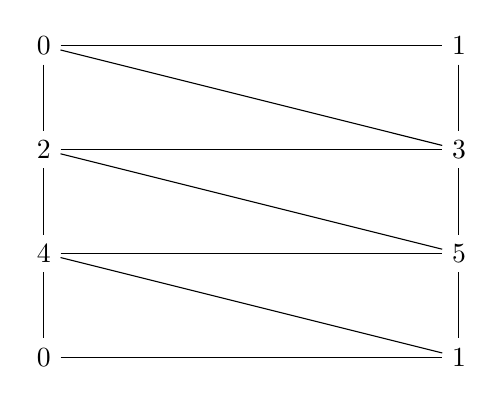
\begin{tikzpicture}[x=0.75pt,y=0.75pt,yscale=-1,xscale=1]

        \node (zero) at (0,0){0};
        \node (one) at (200,0){1};
        \node (two) at (0,50){2};
        \node (three) at (200,50){3};
        \node (four) at (0,100){4};
        \node (five) at (200,100){5};
        \node (zero1) at (0,150){0};
        \node (one1) at (200,150){1};

        \draw (zero) -- (one);
        \draw (two) -- (three);
        \draw (four) -- (five);
        \draw (zero1) -- (one1);
        
        \draw (zero) -- (two) -- (four) -- (zero1);
        \draw (one) -- (three) -- (five) -- (one1);
        
        \draw (zero) -- (three);      
        \draw (two) -- (five); 
        \draw (four) -- (one1);

        \end{tikzpicture}
    \end{center}
\end{figure}

\end{proof}

\noindent\linia

\begin{exercise}
    What are the Euler characteristics of Examples 4.5 and 4.6? What is the Euler characteristic of the icosahedron?
\end{exercise}

\begin{proof}

\textbf{Exemplo 4.5:} 
$$K = \{[0], [1], [2], [3], [0, 1], [1, 2], [2, 3], [3, 0], [0, 2], [1, 3], [0, 1, 2], [0, 1, 3], [0, 2, 3], [1, 2, 3]\}.$$
$$
\chi (K) = 4 - 6 + 4 = 2
$$

\textbf{Exemplo 4.6:}
\begin{multline*}
    K = \{[0], [1],[2], [3], [0, 1], [1, 2], [1,3], [0,2] ,[2, 3], [3, 0], \\
    [0, 1, 2], [0, 1, 3], [0, 2, 3], [1, 2, 3], [0, 1, 2, 3]\}.    
\end{multline*}
$$
\chi (K) = 4 - 6 + 4 - 1 = 1
$$

\textbf{D20:} It has 20 faces (dimension 2), 30 edges (dimension 1) and 12
vertices (dimension 0), its Euler characteristic is $12 - 30 + 20 = 2$ (Euler
relation).

\end{proof}

\noindent\linia

\begin{exercise}
    Let $K$ be a simplicial complex (with vertex set $V$). A sub-complex of
    $K$ is a set $M \subset K$ that is a simplicial complex. Suppose that
    there exists two sub-complexes $M$ and $N$ of $K$ such that $K = M \cup
    N$. Show the inclusion-exclusion principle:
    $$
    \chi(K) = \chi(M) + \chi(N) - \chi(M \cap N)
    $$
\end{exercise}

\begin{proof}

Denote $k_i$ the number of simplices of dimension $i$, that is, $\chi (K) =
\sum_{0 \le i \le k} (-1)^i k_i$, with $k$ being its dimension. Each simplex of dimension $i$ belongs to
$M$, to $N$ or both. Denote $k_i^M, k_i^N$ and $k_i^{MN}$ the number od
simplices of dimension $i$ in $M$, $N$ and $M \cap N$ respectively. So
$$k_i = k_i^M + k_i^N - k_i^{MN}.$$
Therefore, 
$$
\chi(K) = \sum_{0 \le i \le k} (-1)^i (k_i^M + k_i^N - k_i^{MN}) = \sum_{0 \le i \le k}(-1)^i k_i^M + \sum_{0 \le i \le k}(-1)^i k_i^N - \sum_{0 \le i \le k}(-1)^i k_i^{MN} 
$$
Let $m$ and $n$ be the dimension of $M$ and $N$,
respectively. Now I shall prove $M \cap N$ is a simplicial complex. Take
$\sigma \subset M \cap N$ and $\tau \subset \sigma$, then $\tau \subset \sigma
\in M$ and $\tau \subset \sigma \in N$, what implies $\tau \in M \cap N$. It
proves its a simplicial complex with dimension $p$. We know the dimension of $M$ is
$m$, so it implies that for all $i > m$, $k_i^M = 0$. Suppose not and let $k_j^M > 0$ for
some $j > m$, we would have a simplex with dimension greater or equal than
$m$. This is a contradiction, because the the dimension of $M$ is the maximum
dimension of its simplices. This holds for $N$ and $M \cap N$. 
$$
\chi(K) = \sum_{0 \le i \le k} (-1)^i (k_i^M + k_i^N - k_i^{MN}) = \sum_{0 \le i \le k}(-1)^i k_i^M + \sum_{0 \le i \le k}(-1)^i k_i^N - \sum_{0 \le i \le k}(-1)^i k_i^{MN} 
$$
We conclude that 
$$
\chi(K) = \sum_{0 \le i \le m}(-1)^i k_i^M + \sum_{0 \le i \le n}(-1)^i k_i^N - \sum_{0 \le i \le p}(-1)^i k_i^{MN} = \chi(M) + \chi(N) - \chi(M \cap N)
$$
    
\end{proof}

\noindent\linia

\begin{exercise}
    What is the Euler characteristic of a sphere of dimension 1? 2? 3? 
\end{exercise}

\begin{proof}

We may find the Euler characteristic of one triangulation of the sphere. So we
first need to find a triangulation for the sphere $\sphere_n \subset
\R^{n+1}$. We can think in the simplex in this space. In $\R^2$ it's the
triangle, in  $\R^3$ it's the tetrahedron, in $\R^4$ it's the 5-cell and so
on. The simplex in $\R^{n+1}$ has $n + 2$ vertices and each vertex connect to
all the other. We have also $n+2$ simplices of dimension $n$, because each
has $n+1$ points, that is, $\genfrac(){0pt}{}{n+2}{n+1} = n+2$. For each of them, we
must include all its subsets. 

Now we can calculate the Euler characteristic for each triangulation and
therefore each sphere. 

$$
\chi(\sphere_1) = -3 + 3 = 0 
$$
$$
\chi(\sphere_2) = 4 - 6 + 4 = 2 
$$
$$
\chi(\sphere_3) = -5 + 10 - 10 + 5 = 0  
$$
$$
\chi(\sphere_4) = 6 - 15 + 20 - 15 + 6 = 2  
$$

    
\end{proof}

\noindent\linia

\begin{exercise}
    Using the previous exercise, show that $\R^3 - \{0\}$ and $\R^4 - \{0\}$ are not homotopy equivalent.
\end{exercise}

\begin{proof}

Suppose that $\R^3 - \{0\}$ and $\R^4 - \{0\}$ are homotopy equivalent. By
Example 3.15, $\sphere_{n-1}$ is homotopic equivalent to $\R^n - \{0\}$. By
this and using the transitive property we conclude that $\sphere_2$ and
$\sphere_3$ are homotopic equivalent. If that is true, we infer that they have
the same Euler characteristic, what is a contraction by the last exercise.
Hence $\R^3 - \{0\}$ and $\R^4 - \{0\}$ are not homotopy equivalent.

\end{proof}

\noindent\linia

The computational exercises (22 - 26) can be found in the
Github\footnote{\url{github.com/lucasmoschen/topological-data-analysis/blob/main/tutorials/tutorial-1.ipynb}}

\begin{exercise}
    Build triangulations of the letters of the alphabet, and compute their Euler characteristic.
\end{exercise}

\begin{exercise}
    For every $n$, triangulate the bouquet of $n$ circles (see below). Compute
    their Euler characteristic.
\end{exercise}

\begin{exercise}
    Implement the following triangulation of the torus.
\end{exercise}

\begin{exercise}
    Consider the following dataset of 30 points $x_0, ..., x_{29}$ in $R^2$.

    Write a function that takes as an input a parameter $r \ge 0$, and returns
    the simplicial complex $\mathcal{G}(r)$ defined as follows:
    \begin{enumerate}
        \item the vertices of $\mathcal{G}(r)$ are the points $x_0, ..., x_{29}$,
        \item for all $i, j \in [[0, 29]]$ with $i \neq j$, the edge $[i, j]$ belongs to $\mathcal{G}(r)$ if and only if
        $||x_i - x_j|| \le r$.
    \end{enumerate}
    
    Compute the number of connected components of $\mathcal{G}(r)$ for several
    values of $r$. What do you observe?
\end{exercise}

\begin{exercise}
    A Erdos–Renyi random graph $\mathcal{G}(n, p)$ is a simplicial complex
    obtained as follows:
    \begin{enumerate}
        \item add $n$ vertices $1, ..., n$,
        \item for every $a, b \in [[1, n]]$, add the edge $[a, b]$ to the complex with probability $p$.
    \end{enumerate}

    Builds a function that, given $n$ and $p$, outputs a simplicial complex $\mathcal{G}(n, p)$. Observe
    the influence of $p$ on the number of connected components of $\mathcal{G}(10, p)$ and $\mathcal{G}(100, p)$.
\end{exercise}

\newpage

\section{Homological algebra}

\subsection{Important Definitions}

\begin{definition}
    Let $K$ be a simplicial complex. For any $n \ge 0$, define the sets
$$K_n = \{\sigma \in K, dim(\sigma) \le n\}$$
$$K_{(n)} = \{\sigma \in K, dim(\sigma) = n\}.$$
The first set is a simplicial complex, called the n-skeleton of $K$.
\end{definition}

\begin{definition}
    Let $n \ge 0$. The n-chains of $K$ is the set $C_n(K)$ whose elements are
    the formal sums
    $$\sum_{\sigma  \in K_{(n)}} \epsilon_{\sigma}\cdot \sigma \text{ where }
    \forall \sigma \in K_{(n)}, \epsilon_{\sigma} \in \Z/2\Z.$$
    We can give $C_n(K)$ a group structure via
    $$
    \sum_{\sigma \in K_{(n)}} \epsilon_{\sigma} \cdot \sigma + \sum_{\sigma \in K_{(n)}} \eta_{\sigma} \cdot \sigma = \sum_{\sigma \in K_{(n)}} (\epsilon_{\sigma} + \eta_{\sigma}) \cdot \sigma.$$
\end{definition}

\begin{definition}
    Let $n \ge 1$, and $\sigma \in K_{(n)}$ a simplex of dimension $n$. We
    define its boundary as the following element of $C_{n-1}(K)$:
    $$
    \partial_n \sigma = \sum_{\tau \subset \sigma, |\tau| = |\sigma| - 1} \tau
    $$ and 
    $$
    \partial_n \sum_{\sigma \in K_{(n)}} \epsilon_{\sigma} \cdot \sigma  =  \sum_{\sigma \in K_{(n)}} \epsilon_{\sigma} \cdot \partial_n \sigma 
    $$
\end{definition}

\begin{definition}
    We define
    \begin{enumerate}
        \item The n-cycles: $Z_n(K) = Ker(\partial_n)$,
        \item The n-boundaries: $B_n(K) = Im(\partial_{n+1}).$
    \end{enumerate}
    We say that two chains $c, c' \in C_n(K)$ are homologous if there exists
    $b \in B_n(K)$ such that $c = c' + b$.
\end{definition}

\begin{definition}
    The $n^{th}$ homology group of $K$ is $H_n(K) = Z_n(K)/B_n(K)$.
\end{definition}

\begin{definition}
    Let $K$ be a simplicial complex and $n \ge 0$. Its $n^{th}$ Betti number
    is the integer $\beta_n(K) = dim~ H_n(K)$.
\end{definition}

\begin{definition}
    The homology groups of a topological space are the homology groups of any triangulation of it. We define their Betti numbers similarly.
\end{definition}

\subsection{Exercises}

\begin{exercise}
    Let $V$ be a $\Z/2\Z$-vector space, and $W$ a linear subspace. Prove that
    $$\text{dim } V /W = \text{dim } V - \text{dim } W  .$$
\end{exercise}

\begin{proof}

Suppose $V$ is finite-dimensional, such that $dim ~V = n + m$ and $dim ~W =
m$. As we have a finite basis and a finite field, we only have finite
number of combinations from the vector of this basis. In special $V$ is finite. By Proposition 5.2,
$V$ has cardinal $2^{m+n}$ and $W$ has cardinal $2^m$. Let's prove that $V/W$
has cardinal $2^n$. We know the quotient space has finite dimension $k$, because
it's finite. So it has $2^k$ elements. Let $V/W = \{[v_1], ..., [v_{2^k}]\}$ where
$v_i$ represents an equivalence class. We know for each $v \in V$ there
exists $i$ such that $v \in v_i + W$ and there is $w \in W$ with $x =
v_i + w$. As each class is disjoint, we first choose one of the $2^k$ classes
$v_i$. After we pick out one element of this class. We have $2^m$ elements in
$W$. Let's see $|v_i + W| = 2^m$. Take $w, w' \in W$ and  suppose $v_i + w =
v_i + w'$. Summing $v_i$ in both sides we obtaing that $w = w'$. So we have
$2^k 2^m$ ways
of forming elements os $V$. We conclude $k$ must be $n$, what finishes our proof. 

\begin{remark}
    Consider the following proof slightly more general. 
\end{remark}

Suppose $V$ is finite-dimensional and let $\{w_1, ..., w_m\}$ be a basis of
$W$. So we can extend this to a basis on $V$, namely, $\{w_1, ..., w_m, v_1,
..., v_{n}\}$, where, $\text{dim } V = m + n$. Consider the set $\{v_1 + W, ...,
v_n + W\}.$ First, let's prove it's free.
$$
0 + W = \sum_{j=1}^n \lambda_j(v_j + W) = \left(\sum_{j=1}^n \lambda_j v_j \right) + W, 
$$
So $\left(\sum_{j=1}^n \lambda_j v_j \right) \in W$. But it implies it can be
written as a linear combination of $\{w_1, ..., w_m\}$, what contradicts the
fact that $\{w_1, ..., w_m, v_1,
..., v_{n}\}$ is linear independent. 

Now take $v + W \in V/W$, where $v = \sum_{j=1}^m \lambda_j w_j + \sum_{j=1}^n
\lambda_{j+m} v_j$. So 
\begin{equation*}
    \begin{split}
        v + W &= \left[\sum_{j=1}^m \lambda_j w_j + \sum_{j=1}^n
        \lambda_{j+m} v_j\right] + W \\
        &= \sum_{j=1}^m \lambda_j (w_j + W) + \sum_{j=1}^n
        \lambda_{j+m} (v_j+ W) \\
        &= \sum_{j=1}^n
        \lambda_{j+m} (v_j+ W) 
    \end{split}
\end{equation*}

We conclude $\{v_1,
..., v_{n}\}$ is a basis what implies $\text{dim } V/W = n = m + n - m$. 

\end{proof}

\noindent\linia

\begin{exercise}
    Let $(G, +)$ be a group, potentially non-commutative. Prove that
    $$\forall g \in G, g + g = 0 \implies G \text{ is commutative.}$$
\end{exercise}

\begin{proof}

Let $u,v \in G$. So $u + v + v = u + (v + v) = u + 0 = u$. With that in mind,
we see that 
$$
u + v + v + u = 0 \implies (u + v) + (v + u) = 0 
$$
We know $v + u$ and $u + v$ are elements of $G$. So we can add to each side
and obtain 
$$
(u + v) + (v + u) + (v + u) = (v + u) \implies u + v = v + u
$$
As $u$ and $v$ are arbitrary, $G$ is commutative. 

\end{proof}

\noindent\linia

\begin{exercise}
    Compute the Betti numbers $\beta_0(K), \beta_1(K)$ and $\beta_2(K)$ of the
    following simplicial complex:
    $$
    K = \{[0], [1], [2], [3], [0, 1], [1, 2], [2, 3], [3, 0]\}.
    $$
\end{exercise}

\begin{proof}

$Z_0(K) = C_0(K)$

$B_0(K) = \{[0] + [1], [1] + [2], [2] + [3], [3] + [0], [0] + [2], [1] + [3],
[0] + [1] + [2] + [3], 0\}$

As $B_0$ have $2^3$ elements and $Z_0$ has $2^4$, we deduce that 
$$\beta_0(K) = dim ~Z_0(K) - dim ~B_0(K) = 4 - 3 = 1$$

$Z_1(K) = \{[0,1] + [1,2] + [2,3] + [3,0], 0\}$

$B_1(K) = \{0\}$

Nesse caso, observamos que, utilizando a mesma ideia do ponto anterior 
$$\beta_1(K) = 1 - 0 = 1.$$
$$
K = \{[0], [1], [2], [3], [0, 1], [1, 2], [2, 3], [3, 0]\}.
$$
$Z_2(K) = \{0\}$

$B_2(K) = \{0\}$

Portanto $\beta_2(K) = 0$. 

\end{proof}

\noindent\linia

\begin{exercise}
    Compute the Betti numbers $\beta_0(K), \beta_1(K)$ and $\beta_2(K)$ of the
    following simplicial complex:
    $$
    K = \{[0], [1], [2], [3], [0, 1], [1, 2], [2, 3], [3, 0], [0, 2], [1, 3], [0, 1, 2], [0, 1, 3], [0, 2, 3], [1, 2, 3]\}.
    $$
\end{exercise}

\begin{proof}

$Z_0(K) = C_0(K)$

$B_0(K) = \{[0] + [1], [1] + [2], [2] + [3], [3] + [0], [0] + [2], [1] + [3],
[0] + [1] + [2] + [3], 0\}$

As $B_0$ have $2^3$ elements and $Z_0$ has $2^4$, we deduce that 
$$\beta_0(K) = dim ~Z_0(K) - dim ~B_0(K) = 4 - 3 = 1$$

\begin{multline}
    Z_1(K) = \{[0,1] + [1,2] + [0,2]; [0,1] + [0,3] + [1,3]; [0,2] + [2,3] +
    [0,3]; \\ 
    [1,2] + [2,3] + [1,3]; [0,1] + [1,2] + [2,3] + [0,3]; [0,1] + [1,3] + [2,3] + [2,0]; \\
    [0,2] + [1,2] + [1,3] + [0,3]; 0
    \}    
\end{multline}
\begin{multline}
    B_1(K) = \{[0,1] + [1,2] + [0,2]; [0,1] + [0,3] + [1,3]; [0,2] + [2,3] +
    [0,3]; \\ 
    [1,2] + [2,3] + [1,3]; 
    [0,1] + [1,2] + [2,3] + [0,3]; [0,1] + [1,3] + [2,3] + [0,2]; \\
    [0,2] + [1,2] + [1,3] + [0,3]; 0
    \}    
\end{multline}

Observe que os conjuntos são iguais e, portanto, 
$$\beta_1(K) = 0.$$

$Z_2(K) = \{[0,1,2] +[0,1,3] + [0,2,3] + [1,2,3], 0\}$

$B_2(K) = \{0\}$

Portanto $\beta_2(K) = 1$. 

\end{proof}

\newpage

\section{Incremental algorithm}

\subsection{Important definitions}

\begin{definition}
    Let $i \in [[1, n]]$, and $d = dim(\sigma_i)$. The simplex $\sigma_i$ is
    positive if there exists a cycle $c \in Z_d(K^i$ ) that contains
    $\sigma_i$. Otherwise, $\sigma_i$ is negative.
\end{definition}

\begin{definition}
    Defines for a set $V = \{0,1,...,n\}$ a simplicial complex 
    $$
    \Delta_n = \{S \subset C, S \neq \emptyset\}
    $$
    and call it simplicial standard n-simplex with boundary 
    $$
    \partial \Delta_n = \Delta_n/V
    $$
\end{definition}

\begin{definition}
    Define the boundary matrix of $K$, denoted $\Delta$ as follows:
    $\Delta$ is a $n \times n$ matrix, whose 
    $$\Delta_{i,j} = \begin{cases}
    1, &\text{if }\sigma_i \subset \sigma_j \text{ and } |\sigma^i| =
    |\sigma^j| - 1 \\
    0, &\text{else} 
    \end{cases}$$
\end{definition}

\subsection{Exercise}

\begin{exercise}
    Compute again the Betti numbers of the simplicial complexes of Exercises 29 and 30, using the incremental algorithm.
\end{exercise}

\begin{enumerate}
    \item    $K = \{[0], [1], [2], [3], [0, 1], [1, 2], [2, 3], [3, 0]\}.$
    
    First we determine the ordering to be as placed in the set. It fulfills the
    required property. After, we find the signals for it $\sigma^i$. The first
    four elements are positive, because, $\partial_0$ has $C_0(K^i)$ as
    kernel. On the other hand $[0,1]$, $[1,2]$ and $[2,3]$ are negatives. At
    last $[3,0]$ is positive, because $[0,1] + [1,2] + [2,3] + [3,0]$ belongs
    to $Z_1(K^8)$. Now we can follow the algorithm thorough a table: 

    \begin{center}
        \begin{tabular}{ c|c|c|c|c|c|c|c|c}
         - & $\sigma^1$ & $\sigma^2$ & $\sigma^3$ & $\sigma^4$ & $\sigma^5$ &
         $\sigma^6$ & $\sigma^7$ &$\sigma^8$ \\ 
         \hline
         Signal & + & + & + & + & - & - & - & + \\  
         $\beta_0(K)$ & 1 & 2 & 3 & 4 & 3 & 2 & 1 & 1 \\ 
         $\beta_1(K)$ & 0 & 0 & 0 & 0 & 0 & 0 & 0 & 1\\     
         $\beta_2(K)$ & 0 & 0 & 0 & 0 & 0 & 0 & 0 & 0\\     

        \end{tabular}
    \end{center}

    \item  $K = \{[0], [1], [2], [3], [0, 1], [1, 2], [2, 3], [3, 0], [0, 2], [1, 3], [0, 1, 2], [0, 1, 3], [0, 2, 3], [1, 2, 3]\}.
    $
    
    First we determine the ordering to be as placed in the set. It fulfills
    the required property. After, we find the signals for it $\sigma^i$.  The vertices have positive signal. The following three edges cannot form any cycle, so they are negative. The last three edges are part of a cycle considering three other already placed of its dimension. When we achieve the simplices with dimension 2, the first three must be negative, because when we sum every combination of them, the boundary has image different from 0. The last, however will be positive.  
    Now we can follow the algorithm thorough a table: 

    \begin{center}
        \begin{tabular}{ c|c|c|c|c|c|c|c|c|c|c|c|c|c|c}
         - & $\sigma^1$ & $\sigma^2$ & $\sigma^3$ & $\sigma^4$ & $\sigma^5$ &
         $\sigma^6$ & $\sigma^7$ &$\sigma^8$ &$\sigma^9$ &$\sigma^{10}$
         &$\sigma^{11}$ &$\sigma^{12}$ &$\sigma^{13}$ &$\sigma^{14}$ \\ 
         \hline
         Signal & + & + & + & + & - & - & - & + & + & + & - & - & - & + \\  
         $\beta_0(K)$ & 1 & 2 & 3 & 4 & 3 & 2 & 1 & 1 & 1 & 1 & 1 & 1 & 1 & 1\\ 
         $\beta_1(K)$ & 0 & 0 & 0 & 0 & 0 & 0 & 0 & 1 & 2 & 3 & 2 & 1 & 0 & 0 \\     
         $\beta_2(K)$ & 0 & 0 & 0 & 0 & 0 & 0 & 0 & 0 & 0 & 0 & 0 & 0 & 0 & 1\\     

        \end{tabular}
    \end{center}

\end{enumerate}

The result corroborates with those found previously. 

\noindent\linia

\begin{exercise}
    Prove that $\partial \Delta_n$ is a triangulation of the $(n -1)$-sphere
    $\sphere_{n-1} \subset \R^n$. 
\end{exercise}

\textcolor{red}{It's clear that $\partial \Delta_n$ is a simplicial complex, because, for
every simplex $\sigma \in \partial \Delta_n$ and $\tau \subset \sigma$, $\tau
\in \Delta_n$, because its a simplicial complex and $\tau \neq V$, then $\tau
\in \partial \Delta_n$. I shall prove that $|\partial \Delta_n|$, the
topological realization of the set, is homeomorphic to the sphere. 
We can describe the convex hull of boundary of the simplex as 
$$
B_n :=|\partial \Delta_n| = \{(\alpha_0, ..., \alpha_n) \in [0,1]^{n+1}, \sum_{i=0}^n \alpha_i = 1 \text{ and for some } i, \alpha_i = 0\}
$$
Let $H = \{(x_0, ..., x_n) \in \R^{n+1} | \sum_{i=0}^n x_i = 1\}$. It's clear
that $B_n \subset H$. I claim $H$ is homeomorphic to $\R^n$. Define
$f: \R^n \to H$ to be $f(x_1, ...,x_n) = (1 - \sum_{i=1}^n x_i, x_1, ...,
x_n)$. Let's prove it is injective. Take two points in the hyperplane such
that 
$$
(1 - \sum_{i=1}^n x_i, x_1, ...,
x_n) = (1 - \sum_{i=1}^n y_i, y_1, ...,
y_n) \implies y_1 = x_1, ..., y_n = x_n
$$
what proves $f$ is injective. Take $y = (y_0, ..., y_n) \in H$ and define $x =
(y_1, ..., y_n)$, then $f(x) = (1 - \sum_{i=1}^n y_i, y_1, ..., y_n) = (y_0,
..., y_n) = y$ and $f$ is surjective. Extend the $H$ to $\R^{n+1}$ in order to
prove $f$ is continuos with $\epsilon$-$\delta$. Suppose $x = (x_1, ..., x_n)
\in \R^n$ and $\epsilon > 0$. Let $\delta = \epsilon/2 $ and suppose $||x - y|| <
\delta$. By the equivalence of the norms, I can use the norm 1 to prove it. Then
\begin{equation*}
    \begin{split}
        ||f(x) - f(y)|| &= |\sum_{i=1}^n (y_i - x_i)| + |x_1 - y_1| + ... + |x_n - y_n| \\
        &\le \sum_{i=1}^n |y_i - x_i| + \sum_{i=1}^n |y_i - x_i| \\
        &= 2||x - y|| < 2\delta = \epsilon
    \end{split}
\end{equation*}
and $f$ is continuos. Because of that, when we restrict the image of $f$, it
will remain continuos. Let's do it with the inverse extended defined as
$$
g(x_0, ..., x_n) = (x_1,...,x_n)
$$
Take $x = (x_0,...,x_n) \in R^{n+1}$ and $\epsilon > 0$. Let $\delta =
\epsilon$ and suppose $||x-y||<\delta$. So 
\begin{equation*}
    \begin{split}
        ||g(x) - g(y)|| &= |x_1 - y_1| + ... + |x_n - y_n| \\
        &\le |x_1 - y_1| + ... + |x_n - y_n| + |x_0 - y_0| \\
        &= ||x-y|| < \epsilon
    \end{split}
\end{equation*}
So $g$ is also continuos. In particular $g$ restricted to $H$ is also
continuos and it's equal to $f^{-1}$. Therefore $f$ is a Homeomorphism.
Because of that $\sphere_{n-1}$ is homeomorphic to $f(\sphere_{n-1})$. Let's
prove $f(\sphere_{n-1})$ is homeomorphic to $\sphere_n \cap H$.}

\noindent\linia

\begin{exercise}
    Show that the algorithm stops after a finite number of steps.
\end{exercise}

Consider the algorithm

\begin{algorithm}[H]
    \SetAlgoLined
    \KwIn{a boundary matrix $\Delta$}
    \KwOut{a reduced matrix $\tilde{\Delta}$}
     \For(){$j \leftarrow 1$ to $n$}{
        \While(){$\exists i < j$ such that $\delta(i) = \delta(j)$}{
            add column $i$ to column $j$
        }
     }
     \caption{Reduction of the boundary matrix}
    \end{algorithm}

\begin{remark}
    I'd add a condition in the algorithm for undefined $\delta(i)$, that is,
    we should consider the values in the domain of $\delta$.
\end{remark}

I have to prove that for every $1 \le j \le n$, the \texttt{while} block stops
after a finite number of steps. That is, in a finite number of steps $\forall
i < j, \delta(i) \neq \delta(j)$. Fix $j$ and let's prove by induction. First
suppose $k = \delta(j-1) = \delta(j)$. That means $1 = \Delta_{k,j-1} =
\Delta_{k,j}$ and $\Delta_{s,j-1} = \Delta_{s,j}=0, s > k$. When we add
columns $j-1$ and $j$, we will have $\Delta_{k,j} = 0$ and for all $s > k,
\Delta(s, j) = 0$. Therefore $\delta(j) < \delta(j-1)$. Now, suppose that if for
some $l \le i < j, \delta(i) = \delta(j)$,  then we can
do $\delta(j) \neq \delta(i), l \le i < j$ in a finite sequence of steps. If $\delta(l-1) = \delta(j)$, with one step we obtain $\delta(j) <
\delta(l-1)$ and we can have two cases: if $\delta(i) = \delta(j)$, for some
$l \le i < j$ and by the
induction hypotheses, in a finite number os steps one can achieve the desired
property; or if $\delta(i) \neq \delta(j), l-1 \le i < j$. That case needs no
further internal step. In the limit we will have the case when $l=1$ and we
have finite steps to achieve there. We passed the case where $1 = \delta(j) =
\delta(i)$. In this case, $\delta(j)$ turns to be the 0-column and becomes
undefined. By the remark, we break the \texttt{while}. Since we have only
finite values for $j$, the algorithm ends in a finite number of steps. 

\noindent\linia 

\begin{exercise}
    Apply Algorithm to solve Exercise 31.
\end{exercise}

So as to solve both exercises, the order will be as placed in the set for each
case.
After we build the boundary matrix and apply the Algorithm from the last
exercise to obtain the reduced matrix and with it, define $\sigma^i$ as negative
if $\delta(i)$ is defined and positive, otherwise. 

\begin{enumerate}
    \item    $K = \{[0], [1], [2], [3], [0, 1], [1, 2], [2, 3], [3, 0]\}.$
    
    This is the boundary matrix

    \begin{center}
        \begin{tabular}{|c|c|c|c|c|c|c|c|c|}
        \hline
        -          & $\sigma_1$ & $\sigma_2$ & $\sigma_3$ & $\sigma_4$ & $\sigma_5$ & $\sigma_6$ & $\sigma_7$ & $\sigma_8$ \\ \hline
        $\sigma_1$ & 0          & 0          & 0          & 0          & 1          & 0          & 0          & 1          \\ \hline
        $\sigma_2$ & 0          & 0          & 0          & 0          & 1          & 1          & 0          & 0          \\ \hline
        $\sigma_3$ & 0          & 0          & 0          & 0          & 0          & 1          & 1          & 0          \\ \hline
        $\sigma_4$ & 0          & 0          & 0          & 0          & 0          & 0          & 1          & 1          \\ \hline
        $\sigma_5$ & 0          & 0          & 0          & 0          & 0          & 0          & 0          & 0          \\ \hline
        $\sigma_6$ & 0          & 0          & 0          & 0          & 0          & 0          & 0          & 0          \\ \hline
        $\sigma_7$ & 0          & 0          & 0          & 0          & 0          & 0          & 0          & 0          \\ \hline
        $\sigma_8$ & 0          & 0          & 0          & 0          & 0          & 0          & 0          & 0          \\ \hline
        \end{tabular}
    \end{center}

    When we apply the algorithm, we start in $i = 5$. However we do not enter
    the \texttt{while} block until $j = 8$ when $\delta(7) =
    \delta(8) = 4$. So we sum this columns, after $\sigma_6$ to $\sigma_8$ and
    at last $\sigma_5$ to $\sigma_8$. So $\sigma_8$ will be the 0-column,
    while the other remain unaltered. By this, we obtain the signals in order
    to calculate the Betti numbers. 

    \begin{center}
        \begin{tabular}{ c|c|c|c|c|c|c|c|c}
         - & $\sigma^1$ & $\sigma^2$ & $\sigma^3$ & $\sigma^4$ & $\sigma^5$ &
         $\sigma^6$ & $\sigma^7$ &$\sigma^8$ \\ 
         \hline
         Signal & + & + & + & + & - & - & - & + \\  
         $\beta_0(K)$ & 1 & 2 & 3 & 4 & 3 & 2 & 1 & 1 \\ 
         $\beta_1(K)$ & 0 & 0 & 0 & 0 & 0 & 0 & 0 & 1\\     
         $\beta_2(K)$ & 0 & 0 & 0 & 0 & 0 & 0 & 0 & 0\\     

        \end{tabular}
    \end{center}

    \item  $K = \{[0], [1], [2], [3], [0, 1], [1, 2], [2, 3], [3, 0], [0, 2], [1, 3], [0, 1, 2], [0, 1, 3], [0, 2, 3], [1, 2, 3]\}.
    $
    
    The boundary matrix is larger than the previous one. 

    \begin{center}
        \begin{tabular}{|c|c|c|c|c|c|c|c|c|c|c|c|}
            \hline
            -             & $\sigma_{1,2,3,4}$ & $\sigma_5$ & $\sigma_6$ & $\sigma_7$ & $\sigma_8$ & $\sigma_9$ & $\sigma_{10}$ & $\sigma_{11}$ & $\sigma_{12}$ & $\sigma_{13}$ & $\sigma_{14}$ \\ \hline
            $\sigma_1$    & 0                  & 1          & 0          & 0          & 1          & 1          & 0             & 0             & 0             & 0             & 0             \\ \hline
            $\sigma_2$    & 0                  & 1          & 1          & 0          & 0          & 0          & 1             & 0             & 0             & 0             & 0             \\ \hline
            $\sigma_3$    & 0                  & 0          & 1          & 1          & 0          & 1          & 0             & 0             & 0             & 0             & 0             \\ \hline
            $\sigma_4$    & 0                  & 0          & 0          & 1          & 1          & 0          & 1             & 0             & 0             & 0             & 0             \\ \hline
            $\sigma_5$    & 0                  & 0          & 0          & 0          & 0          & 0          & 0             & 1             & 1             & 0             & 0             \\ \hline
            $\sigma_6$    & 0                  & 0          & 0          & 0          & 0          & 0          & 0             & 1             & 0             & 0             & 1             \\ \hline
            $\sigma_7$    & 0                  & 0          & 0          & 0          & 0          & 0          & 0             & 0             & 0             & 1             & 1             \\ \hline
            $\sigma_8$    & 0                  & 0          & 0          & 0          & 0          & 0          & 0             & 0             & 1             & 1             & 0             \\ \hline
            $\sigma_9$    & 0                  & 0          & 0          & 0          & 0          & 0          & 0             & 1             & 0             & 1             & 0             \\ \hline
            $\sigma_{10}$ & 0                  & 0          & 0          & 0          & 0          & 0          & 0             & 0             & 1             & 0             & 1             \\ \hline
            $\sigma_{11}$ & 0                  & 0          & 0          & 0          & 0          & 0          & 0             & 0             & 0             & 0             & 0             \\ \hline
            $\sigma_{12}$ & 0                  & 0          & 0          & 0          & 0          & 0          & 0             & 0             & 0             & 0             & 0             \\ \hline
            $\sigma_{13}$ & 0                  & 0          & 0          & 0          & 0          & 0          & 0             & 0             & 0             & 0             & 0             \\ \hline
            $\sigma_{14}$ & 0                  & 0          & 0          & 0          & 0          & 0          & 0             & 0             & 0             & 0             & 0             \\ \hline
        \end{tabular}
    \end{center}

    This matrix has several more things to deal. First we make the column
    $\sigma_8$ be a 0-column again. After we make the same to $\sigma_9$,
    being replaced by $\sigma_5 + \sigma_6 + \sigma_9$ and $\sigma_{10}$ by
    $\sigma_6 + \sigma_7 + \sigma_{10}$. We will have  

    \begin{center}
        \begin{tabular}{|c|c|c|c|c|c|c|c|c|c|c|c|}
            \hline
            -             & $\sigma_{1,2,3,4}$ & $\sigma_5$ & $\sigma_6$ & $\sigma_7$ & $\sigma_8$ & $\sigma_9$ & $\sigma_{10}$ & $\sigma_{11}$ & $\sigma_{12}$ & $\sigma_{13}$ & $\sigma_{14}$ \\ \hline
            $\sigma_1$    & 0                  & 1          & 0          & 0          & 0          & 0          & 0             & 0             & 0             & 0             & 0             \\ \hline
            $\sigma_2$    & 0                  & 1          & 1          & 0          & 0          & 0          & 0             & 0             & 0             & 0             & 0             \\ \hline
            $\sigma_3$    & 0                  & 0          & 1          & 1          & 0          & 0          & 0             & 0             & 0             & 0             & 0             \\ \hline
            $\sigma_4$    & 0                  & 0          & 0          & 1          & 0          & 0          & 0             & 0             & 0             & 0             & 0             \\ \hline
            $\sigma_5$    & 0                  & 0          & 0          & 0          & 0          & 0          & 0             & 1             & 1             & 0             & 0             \\ \hline
            $\sigma_6$    & 0                  & 0          & 0          & 0          & 0          & 0          & 0             & 1             & 0             & 0             & 1             \\ \hline
            $\sigma_7$    & 0                  & 0          & 0          & 0          & 0          & 0          & 0             & 0             & 0             & 1             & 1             \\ \hline
            $\sigma_8$    & 0                  & 0          & 0          & 0          & 0          & 0          & 0             & 0             & 1             & 1             & 0             \\ \hline
            $\sigma_9$    & 0                  & 0          & 0          & 0          & 0          & 0          & 0             & 1             & 0             & 1             & 0             \\ \hline
            $\sigma_{10}$ & 0                  & 0          & 0          & 0          & 0          & 0          & 0             & 0             & 1             & 0             & 1             \\ \hline
            $\sigma_{11}$ & 0                  & 0          & 0          & 0          & 0          & 0          & 0             & 0             & 0             & 0             & 0             \\ \hline
            $\sigma_{12}$ & 0                  & 0          & 0          & 0          & 0          & 0          & 0             & 0             & 0             & 0             & 0             \\ \hline
            $\sigma_{13}$ & 0                  & 0          & 0          & 0          & 0          & 0          & 0             & 0             & 0             & 0             & 0             \\ \hline
            $\sigma_{14}$ & 0                  & 0          & 0          & 0          & 0          & 0          & 0             & 0             & 0             & 0             & 0             \\ \hline
        \end{tabular}
    \end{center}

    The next column to deal is $\sigma_{13}$. Summing it with $\sigma_{11}$
    will solve the problem. With $\sigma_{14}$ we need to replace with
    $\sigma_{12} + \sigma_{13} \sigma_{14}$, considering the new
    $\sigma_{13}$. But this will turn $\sigma_{14}$ to be a 0-column. We know,
    then, the signals for each column. 

    \begin{center}
        \begin{tabular}{ c|c|c|c|c|c|c|c|c|c|c|c|c|c|c}
         - & $\sigma^1$ & $\sigma^2$ & $\sigma^3$ & $\sigma^4$ & $\sigma^5$ &
         $\sigma^6$ & $\sigma^7$ &$\sigma^8$ &$\sigma^9$ &$\sigma^{10}$
         &$\sigma^{11}$ &$\sigma^{12}$ &$\sigma^{13}$ &$\sigma^{14}$ \\ 
         \hline
         Signal & + & + & + & + & - & - & - & + & + & + & - & - & - & + \\  
         $\beta_0(K)$ & 1 & 2 & 3 & 4 & 3 & 2 & 1 & 1 & 1 & 1 & 1 & 1 & 1 & 1\\ 
         $\beta_1(K)$ & 0 & 0 & 0 & 0 & 0 & 0 & 0 & 1 & 2 & 3 & 2 & 1 & 0 & 0 \\     
         $\beta_2(K)$ & 0 & 0 & 0 & 0 & 0 & 0 & 0 & 0 & 0 & 0 & 0 & 0 & 0 & 1\\     

        \end{tabular}
    \end{center}

\end{enumerate}

\newpage

\end{document}